\begin{enumerate}
  \item Definiční obor
  \item 1. derivace a 2. derivace
  \item Nulové body
    \begin{itemize}
      \item podezřelé z inflexe (mění se zde znaménko)
      \item zkontrolovat, zda leží v D(f)
    \end{itemize}
  \item Znaménko nulových bodů
    \begin{itemize}
      \item $\cup$ konvexní (+)
      \item $\cap$ konkávní (-)
    \end{itemize}
  \item Interval konvexity, konkávity
  \item Inflexe - inflexní body
    \begin{itemize}
      \item změna konvexity, konkávity
      \item definovaná, spojitá v bodě
      \item $I_1[x_1;y_1]$ a $I_2[x_2;y_2]$
    \end{itemize}

\end{enumerate}
\begin{align*}
  f(x)&=-\frac{x^4}{12}+x^3-4x^2-10x+210
\end{align*}
\hrule
$$D(f)=\mathbb{R}$$
\begin{align*}
  f'(x)&=-\frac{x^3}{3}+3x^2-8x-10\\
  f''(x)&=-(x^3-6x+9)=-(x-4)*(x-2)\\
  &\begin{alignedat}{2}
    \text{nulové body  }\,
    \Biggr|\,
    \begin{alignedat}{2}
      x-4 &=0 \quad x_1 \rightarrow &4 \\
      x-2 &=0 \quad x_2 \rightarrow &2 \\
    \end{alignedat}
    \,\Biggr|
  \end{alignedat}
\end{align*}

\begin{center}
  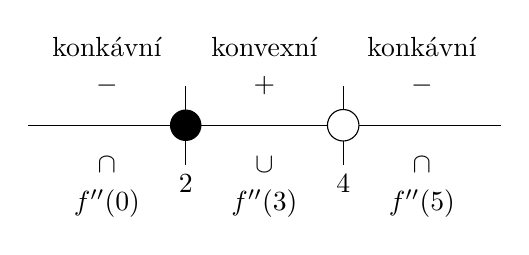
\begin{tikzpicture}[scale=1]
    \draw (-0,0)-- (6,0); %Axis
    \foreach \x in {2,4} {
      \draw (\x,0.5) -- (\x,-0.5) node[below] {\x};
    }
    \fill (2,0) circle (0.2);
    \draw[fill=white] (4,0) circle (0.2);
    \draw (1,1) node{konkávní} (1,0.5) node{$-$} (1,-0.5) node{$\cap$} (1,-1) node{$f''(0)$};
    \draw (3,1) node{konvexní} (3,0.5) node{$+$} (3,-0.5) node{$\cup$} (3,-1) node{$f''(3)$};
    \draw (5,1) node{konkávní} (5,0.5) node{$-$} (5,-0.5) node{$\cap$} (5,-1) node{$f''(5)$};
  \end{tikzpicture}
\end{center}

\begin{center}
  \begin{tabular}{l}
    Konvexní na $\langle2;4\rangle$\\
    Konkávní na $(-\infty;2\rangle$ a $\langle4;\infty)$\\
    Inflexe v $x=2$ a $x=4$\\
    $I_1[2;f(2)]$ a $I_2[4;f(4)]$
  \end{tabular}
\end{center}

\begin{center}
  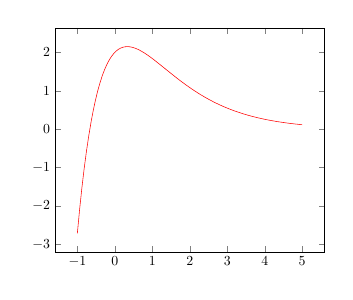
\begin{tikzpicture}[scale=0.5]
    \begin{axis}
      \addplot[color=red,domain=-1:5,samples=100]{(2+3*x)*e^(-x)};
    \end{axis}
  \end{tikzpicture}
\end{center}

